\documentclass[a4paper]{article}

\usepackage[english]{babel} \usepackage[utf8x]{inputenc}
\usepackage{amsmath}
\usepackage{graphicx}
\usepackage[colorinlistoftodos]{todonotes} \usepackage[margin = 1.2in]{geometry}

\title{A Bug's Life}
\author{Oliver Eriksson Edholm (XXXXXX-YYYY) \\
Aleksander Lundqvist (XXXXXX-YYYY) \\
Henrik Sommerland (890618-4950) \\
Edvin Wahlberg (XXXXXX-YYYY) \\
Oscar Wallster(910615-1096)}

\begin{document}
\maketitle

\section{Introduction}
% This could be rewritten in a far more persuasive manner
We have decided that we are going to simpulate an \emph{ant ant}. We want to do
this in order to learn more about both \emph{swarm intelligence} and the actor
model.\\
We choose ants in inspiration of their ability to cooperate in a very large
scale and solve complex problems while still every ant is only following very
simple rules.
\\
Our goal is not to simulate the behaviour of real world ants or to mimick the
datails of any biological systems.
We are more interested in the theorethical concepts of how complex behaviors can
arise from the interaction of a large group of agent each possesing only limited
cognitive abilites.\\

One of the later goals is also to have two or more ant hives interact with
eachother in a world where food is scarce, and battles are inevidieble.

\subsection{Chalenges}

\subsubsection{Concurrency}
Making heavy use of the actor model using thousands of actors will create a lot
of complexity and there are many posibilities for problems to occur. The most
obvious danger is the possibilty of deadlocks to occur. With many actors
comunicating together one is almost certain that one will get some form of
circular dependencies. So great care needs to be taken to ensure that no
deadlocks will occur.

There is also a risk of severe performance degradation in regions with many
interacting actors. Although this is something wich is intrinsic to the actor
model and it may be hard for us to control it.

\subsubsection{Rules For Interaction}
The other chalange will be to setup rules for how the ants interact with the
world and jhow the world gets updated. The parameters for these rules will need
to be finetuned and it may be hard to find rules which result in complex
behaviours. It is also very hard to analytically determine these parameters so
the only feasible alternative is to trough experimentation find rules which
yields satisfactory behavious.

\subsubsection{Social Challanges}
In order to get this project moving forward in a pace that is required, we need
to have every member of the group working regularly certain hours of the weeks.
In order to achieve this every member needs to have the same mental image over
the finished project, therefore we need to be active with communication in the
roup so that noone is left behind and wonders what he could/should be doing.

\section{Concurrency Models and Programming Languages}

\subsection{Concurrency Goals}
As previously stated we want to create a system wich relies heavily on the actor
model. Our project idea is well suited for this since the ants are by nature
individual agents who and make decisions without any direct knowlegde of the
global state.

\subsubsection{No Global Locks}

We want to make our simulation free of so called \emph{stop the world}
sencarios. These are when we for some reason have to block al of the actors in
the simulation in order to perform some kind of action.


\subsection{Rust}

\subsection{Nim}

\subsection{Erlang}

\subsection{Encore}

\section{System Architecture}

\begin{figure}[h!]
\centerline{
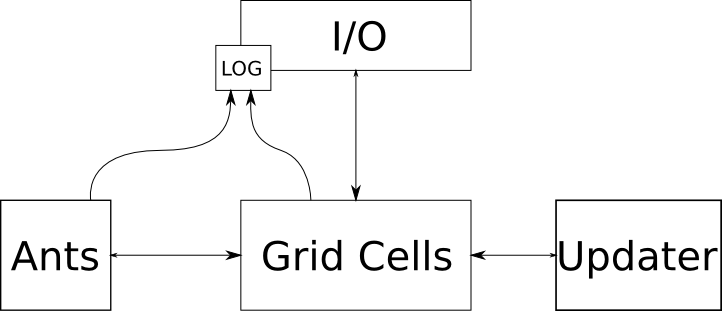
\includegraphics[scale=0.5]{images/architecture.png}
}
\caption{Change in diversity} 
\end{figure}

\section{Development Tools}
In order to achieve this every member needs to have the same mental image over
the finished project, therefore we need to be active with communication in the
group so that noone is left behind and wonders what he could/should be doing.

\section{Development Tools}
Communication and planning: To plan meetings and set up to-do tasks for the
project, we have chosen to use Trello. Trello is very user friendly and will
give us a great overview of the progress of the project. It will also be a good
tool to keep track of who is doing what. For communication we’re going to use
Slack to ensure that we have all communication of the project in one place. If
we should have chosen to use Facebook it’s very easy to get distracted and talk
about other things that isn’t related to the project. If we really need discuss
something urgent we’re going to use Skype.

\section{Conclusion}
Digital ant colonization is perfect project for developing deeper understanding
of the actor model of concurency, since each ant is an independent actor and
only interact with its immidiate surroundings. This project can be divided into
diffrent milestones which can be developed further as time lasts. We all have
alot and diffrent ideas how we want the final product to work, but we all agree
on the basics so as time elapse we will hopefully be able to add alot more
complexity depending how much work will be needed for each milestone. Ergo we
start with a stable core and build outwards in diffrent directions.
\end{document}

